\chapter{数据集}
本章详细描述基于CLEVR数据集,构造本文所用的CLEVR-ASP数据集的过程,以及数据集的设计思路、ASP约束编码规则。
\section{物体属性}
CLEVR-ASP数据集的图像中的每个物体,均有形状、尺寸、材质、颜色四种属性。每种属性的可能取值如下:
\begin{enumerate}[label=(\arabic*),itemsep=0pt,parsep=0pt]
    \item 形状:圆锥体、球体。
    \item 尺寸:小、中、大。
    \item 材质:橡胶、金属。
    \item 颜色:红色、蓝色、绿色、黄色、灰色、棕色。
\end{enumerate}

除了以上四种属性之外,由于图像中的场景被划分成4个区域,故CLEVR-ASP数据集也将图像中的物体按照其所在区域进行划分,
分别标记为0、1、2、3。每个物体都恰好位于某一个区域之中。将图像中的场景划分为多个区域,可以在多个级别上
分别指定约束。

\begin{enumerate}[itemsep=0pt,parsep=0pt]
    \item 区域约束:某个区域内的所有物体必须满足特定属性。例如,所有在区域 0 的物体必须是 立方体或圆柱体。
    \item 夸区域约束:定义了多个区域之间的关系。例如,区域1和区域2内同一个颜色的物体数量之和不得超过2。
    \item 全局约束:其中包含了一组影响整个场景的规则。例如,场景中至少有 2 个立方体。
\end{enumerate}

以上所有约束,使用ASP来进行表示。例如:
\begin{lstlisting}
    :- object(X), at(X, 0), not hasProperty(X, shape, cube), not hasProperty(X, shape, cylinder).
\end{lstlisting}
表示如果 X 在 区域 0,那么它的形状必须是 立方体或圆柱体。

\section{环境表示}
CLEVR-ASP中的一个环境是由一组约束来定义的。每个约束决定了特定环境下物体的属性限制。数据集包含
30个环境,每个环境中最多包含15个不同约束。部分约束的ASP编码表示以及对应表示含义见表\ref{tab:asp_templates}。

\begin{table}[h]
    \centering
    \renewcommand{\arraystretch}{1.2}
    \begin{tabular}{|p{3cm}|p{12cm}|}
        \hline
        \textbf{模板} & \textbf{描述} \\
        \hline
        \textbf{模板1(取值约束)} & 
        \texttt{:- object(X), at(X, R), not hasProperty(X, P1, V1).} \\ 
        & 解释: 对区域R中的所有物体,它们P1属性的取值均为V1。 \\ 
        & 具体实现: $:- object(X), at(X, 0), not hasProperty(X, color, red).$ \\
        \hline
        
        \textbf{模板2(否定约束)} & 
        \texttt{:- object(X), at(X, R), hasProperty(X, P1, V1).} \\ 
        & 解释:对区域R中的所有物体,它们的P1属性的取值,均不能为V1。 \\ 
        & 具体实现::- object(X), at(X, 0), hasProperty(X, material, metal). \\
        \hline
        
        \textbf{模板3(恰有N个约束)} & 
        \texttt{:- \#count\{X: hasProperty(X, P1, V1), object(X), at(X, R)\} != N.} \\ 
        & \textbf{解释}:在区域R中,恰好有N个物体的P1属性的取值为V1。 \\ 
        & 具体实现::- \#count\{X: hasProperty(X, size, small), object(X), at(X, R')\} != 2. \\
        \hline
        
        \textbf{模板4(至少有N个约束)} & 
        \texttt{:- \#count\{X1, X2: sameProperty(X1, X2, P1), object(X1), object(X2), at(X1, R1), at(X2, R2)\} < N.} \\ 
        & 解释:在区域R1和区域R2中,至少有N对物体,它们的P1属性的取值都是V1。 \\ 
        & 具体实现::- \#count\{X1, X2: sameProperty(X1, X2, shape), object(X1), object(X2), at(X1, 1), at(X2, 2)\} < 1. \\
        \hline
        
        \textbf{模板5(或约束)} & 
        \texttt{:- object(X), at(X, R), not hasProperty(X, P1, V1), not hasProperty(X, P1, V2).} \\ 
        & 解释:区域 R中的所有对象都具有属性 P1 的 V1 值或属性 P2 的 V2 值。 \\ 
        & 具体实现::- object(X), at(X, 1), not hasProperty(X, color, yellow), not hasProperty(X, color, blue). \\
        \hline
    \end{tabular}
    \caption{约束模板}
    \label{tab:asp_templates}
\end{table}

\section{场景表示}
CLEVR数据集以场景图的形式表示场景,其节点表示使用其属性进行注释的对象,边表示对象之间的空间关系(前、后、左、右)。在CLEVR-ASP中,除了场景图表示之外,还在ASP中表示一个场景。
下面以图1为例,展示部分场景的ASP表示:
\begin{lstlisting}
%Objects in the scene
object(0). object(1). object(2). object(3).

%Attributes of objects
at(0, 2).
hasProperty(0, color, green).
hasProperty(0, size, large).
hasProperty(0, material, rubber).
hasProperty(0, shape, cylinder).
....

%Spatial relations between objects
front(1, 0). right(1, 0). ...
\end{lstlisting}

谓词\texttt{object}用于定义不同的物体(所有物体的名称用0,1等数字来表示),
\texttt{hasProperty(Object, Attribute, Value)}用于将对象的名为Attribute的属性的值设置为Value。
对象之间的空间关系用谓词\texttt{left}、\texttt{right}、\texttt{front}、\texttt{behind}来表示,例如
\texttt{left(A, B)}表示B位于A的左侧。

\section{图像生成}
虽然CLEVR中的图像是通过随机采样的场景图生成的,
但CLEVR-ASP生成的图像是基于已知符合环境约束的场景图。
场景图的创建因此成为一个推理问题——
在给定环境(基于答案集编程ASP的约束条件)和场景中预期物体数量$n$的前提下,
需要完成以下任务:将每个物体分配到四个区域之一,并为颜色、尺寸、形状和材质属性赋值,确保这些属性符合环境中的约束条件。

解决这一问题,需要ASP求解器来完成。具体而言,ASP求解器将返回一个解集,集合中的
每个答案(即 $n$ 个对象的一个一致属性值分配方案)代表一个场景图,
或者说是场景中物体的一种可能配置。由于可能的配置方案众多,
因此 CLEVR-ASP 随机采样了一百万个场景图用于后续的图像生成阶段。
接下来,使用 Blender3 对场景图进行渲染,最终生成完整场景的图像。
而部分场景的图像则是基于部分场景图生成的,具体做法是从实际场景图中随机移除一个物体,
从而构造部分场景图。图\ref{pipeline_for_generating_environment}展示了场景图的构造过程。
\begin{figure}
    \centering
    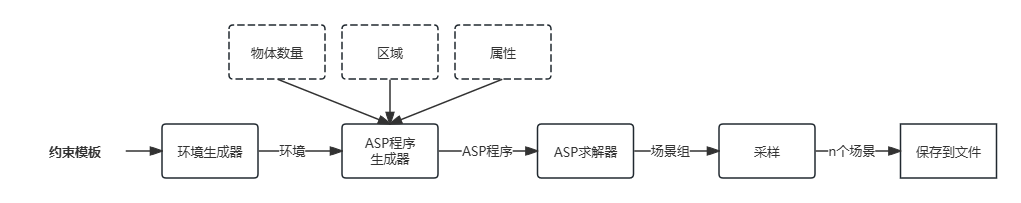
\includegraphics[width=\textwidth]{pipeline_for_generating_environment.png}
    \caption{生成环境以及该环境中的完整场景的流水线}
    \label{pipeline_for_generating_environment}
\end{figure}

\section{问题表示}
CLEVR-ASP中的问题围绕部分场景中缺失的物体的颜色、大小、形状、材质这四个属性之一。
具体的问题实例及ASP编码实例如下:

自然语言问题:与中等大小的红色物体的材质相同的,另一个圆柱体的颜色是什么?
\begin{lstlisting}
    query(Q) :- hasProperty(X, color, Q),
    hasProperty(X, shape, cylinder),

    hasProperty(Y, size, medium),
    hasProperty(Y, color, red),
    same_material(Y, X),
    X != Y.
\end{lstlisting}

如果问题是关于属性$A, A \in \{ color, size, material, shape\}$,那么生成问题时,
可能的解集S的基数为$1 \leq |S| \leq |A|$,其中$|A|$是属性A的所有可能取值集合的大小。例如,$|size| = 3 =\{ large, medium, small\}$
。如果生成的问题有$|A|$个解,那么可判定该问题无效。例如,对于一个问物体尺寸的问题,答案是“尺寸可以为大或者中或者小”,显然这个答案是无效的,因为
对于任意一个尺寸相关的问题,该答案均有效。各种类型的问题在个数上保持平衡。
\section{问题生成}
我们以CLEVR中的问题作为范本,来生成CLEVR-ASP中的问题。生成的问题均关于属性,避免生成是否类问题以及计数类问题。
以下为问题模板样例:
\begin{lstlisting}
What shape is the < Z2 > (size) < C2 > (color) < M2 > (material) [that is] 
< R > (relation) the < Z > (size) < C > (color) < M > (material) < S > (shape) ?
\end{lstlisting}

问题模板的实例化是基于相关图像的完整场景图完成的。
感兴趣的对象始终是从完整场景中移除以生成部分场景图的对象。
查询属性的选择需满足问题类型平衡的要求。
查询对象的已知属性(填充上述模板中的 <Z2>、<C2> 或 <M2> 位置)是随机选取的。
而 <R> 位置(即 left、right、front、behind 之一)的填充值也是随机选择的,
但问题中的参考对象是根据完整场景中的空间关系选择的——具体而言,
从与查询对象存在 <R> 关系的对象中选取一个。

问题的 ASP 表示、部分场景以及环境中的约束都会被提供给 ASP 求解器,
以确定问题的可能解。图\ref{pipeline_for_generating_partial}展示了问题生成的流水线过程。
\begin{figure}
    \centering
    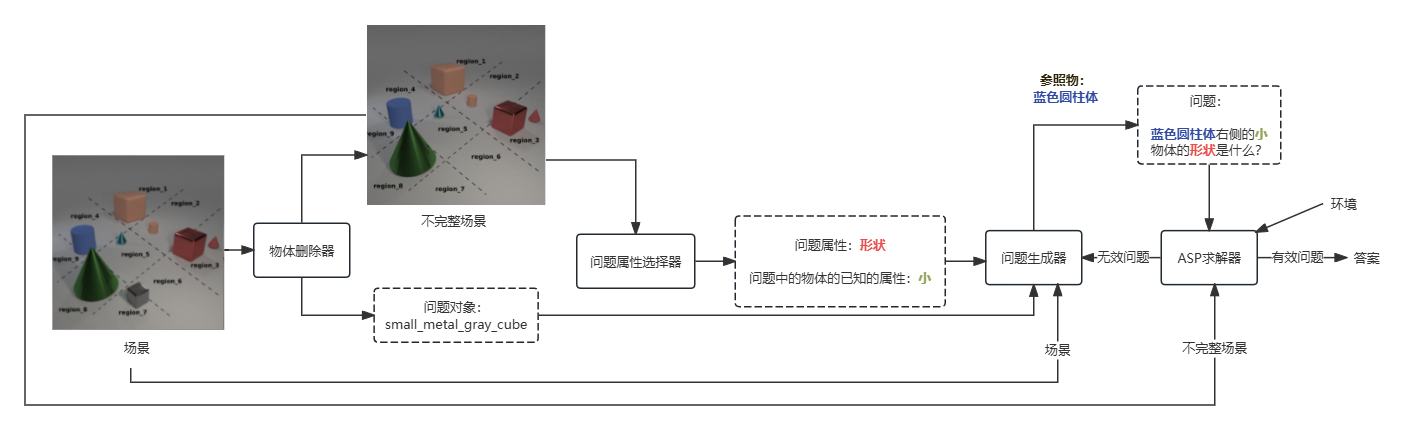
\includegraphics[width=\textwidth]{pipeline_for_generating_partial.png}
    \caption{生成部分场景和问题,并进行标记的流程}
    \label{pipeline_for_generating_partial}
\end{figure}
\section{本章小结}
本章介绍了 CLEVR-ASP 数据集的构造过程,重点描述了如何基于完整场景图生成部分场景图,并通过 ASP(Answer Set Programming)实例化问题模板以确保问题的多样性和合理性。

首先,本章阐述了对象移除的原则,即如何选择查询对象以及如何保证其属性在问题类型上的均衡性。随后,详细说明了查询模板的填充策略,包括查询属性的选取、参考对象的确定以及空间关系的合理性,以确保生成的问题符合实际场景。最后,本章介绍了 ASP 求解器在问题生成过程中的作用,即利用 ASP 规则对部分场景进行推理,以确定查询属性的可能取值范围,从而生成符合逻辑约束的高质量视觉问答数据。

通过上述方法,CLEVR-ASP 数据集不仅保证了问题的可解释性,还增强了对复杂空间关系的推理能力,为视觉问答任务提供了更具挑战性的数据支持。